\documentclass[11pt,a4paper,titlepage]{article}
\usepackage[utf8x]{inputenc}
\usepackage{ucs}
\usepackage{ulem}
\usepackage{amsmath}
\usepackage{amsfonts}
\usepackage{amssymb}
\usepackage{pdfpages}
\usepackage[linkbordercolor={1 1 1}, urlbordercolor={1 1 1}]{hyperref}
\usepackage[german]{babel}
\usepackage{eurosym}
\usepackage{pdfpages}
\usepackage{graphicx}
\usepackage{float}
\setcounter{secnumdepth}{4} 
\setlength{\parindent}{3em}
\usepackage[paper=a4paper,left=15mm,right=15mm,top=20mm,bottom=20mm]{geometry}
\pagestyle{plain} 
\title{{\Huge Exportieren und Importieren von TSM-Daten} \linebreak \linebreak

\includegraphics[width= 35px]{../BilderHandbuch/icon32.png} \\
\textbf{Testsuite-Management\\ (TSM)}}
\author{Tobias Hirning}
\usepackage[space,extendedchars]{grffile}
\begin{document}

\maketitle
\pagebreak

\tableofcontents
\pagebreak

\flushleft
\section{Generelles zum Im- und Exportieren}
Sie können sowohl Testfälle als auch Pakete exportieren und in einer anderen Installation importieren. Dabei ist zu beachten, dass \textbf{Bilder und Protokolle beim Export nicht übernommen werden}.\\
Sollten Sie komplette Projekte ex- und importieren so kann es sein, dass Protokolle dreifach angezeigt werden. \textbf{Der Ex- und Import von Projekten wird nicht empfohlen.} Nutzen Sie dafür Versionsverwaltungssystem um Ihren Arbeitsordner
 ("`workspace"'-Verzeichnis) in verschiedenen Installationen zu nutzen.\\
Im Folgenden wird beschrieben, wie Sie einen Testfall ex- und importieren. Für ein gesamtes Paket gehen Sie analog vor.\\
\vspace{\baselineskip}
\textbf{Achtung, sichern Sie Ihre Daten vor jedem Ex- bzw. Import!}

\section{Testfälle exportieren}
Um einen Testfall zu exportieren selektieren Sie diesen und machen einen Rechtsklick. Im Kontextmenü wählen Sie dann \texttt{Exportieren ...}.
\begin{figure}[H]
 \centering
 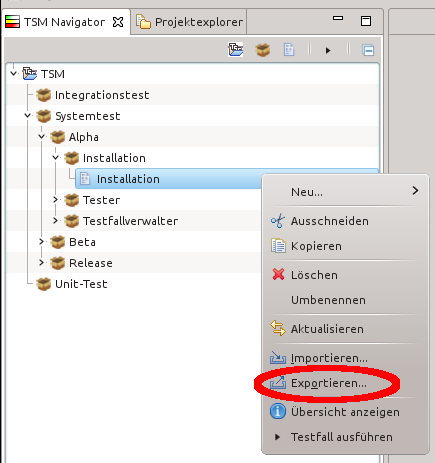
\includegraphics{./kontextmenue-exp.png}
 % kontextmenue-exp.png: 435x463 pixel, 98dpi, 11.28x12.00 cm, bb=0 0 320 340
 \caption{\texttt{Exportieren...} im Kontexmenü.}
 \label{abb:Kontextmenue-exp}
\end{figure}
\vspace{\baselineskip}
Wählen Sie anschließend \texttt{Dateisystem} (1) und klicken Sie auf \texttt{Weiter} (2).
\begin{figure}[H]
 \centering
 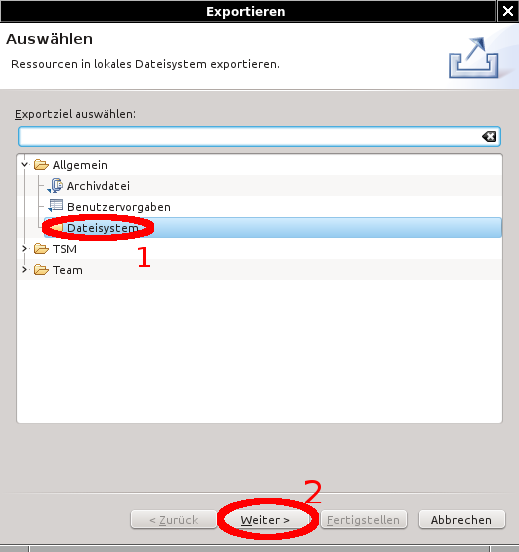
\includegraphics{./assistent-exp1.png}
 % assistent-exp1.png: 519x552 pixel, 98dpi, 13.45x14.31 cm, bb=0 0 381 406
 \caption{\texttt{Dateisystem} und dann \texttt{Weiter}.}
 \label{abb:Assistent-exp1}
\end{figure}
\vspace{\baselineskip}
Anschließend wählen Sie den gewünschten Testfall mit einem Haken aus (1) und wählen \texttt{Verzeichnisstruktur für Dateien erstellen}. Beenden Sie den Export mit einem Klick auf \texttt{Fertigstellen}.
\begin{figure}[H]
 \centering
 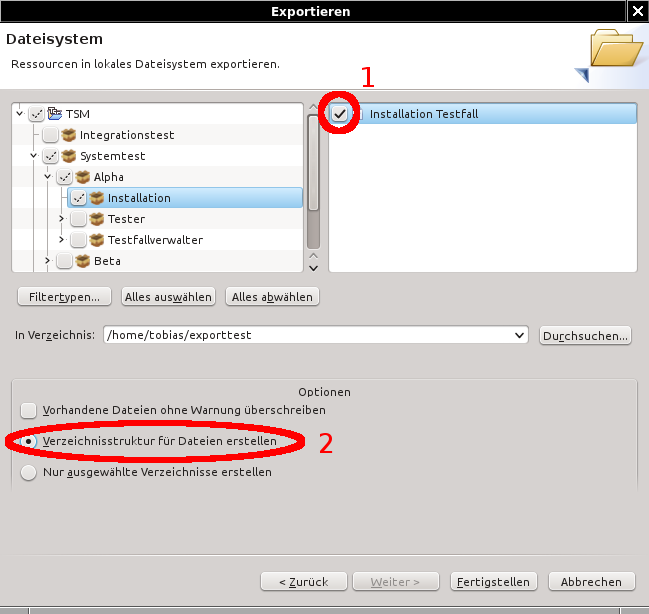
\includegraphics{./assistent-exp2.png}
 % assistent-exp2.png: 649x614 pixel, 98dpi, 16.82x15.91 cm, bb=0 0 477 451
 \caption{Haken setzen und dann \texttt{Verzeichnisstruktur für Dateien erstellen}.}
 \label{abb:Assistent-exp2}
\end{figure}


\section{Testfälle importieren}
Um einen Testfall zu importieren muss bereits ein Projekt vorhanden sein, in das er importiert werden sollen.\\
Selektieren Sie das Projekt und machen Sie einen Rechtsklick darauf. Im Kontextmenü wählen Sie dann \texttt{Importieren...}.
\begin{figure}[H]
 \centering
 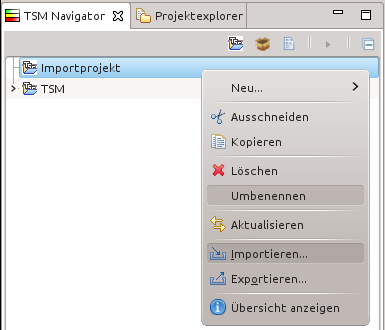
\includegraphics{./kontextmenue-imp.png}
 % kontextmenue-imp.png: 385x330 pixel, 98dpi, 9.98x8.55 cm, bb=0 0 283 242
 \caption{\texttt{Importieren...} im Kontextmenü.}
 \label{abb:Kontextmenue-imp}
\end{figure}
\vspace{\baselineskip}
Wählen Sie anschließend \texttt{Dateisystem} (1) und klicken Sie auf \texttt{Weiter} (2).
\begin{figure}[H]
 \centering
 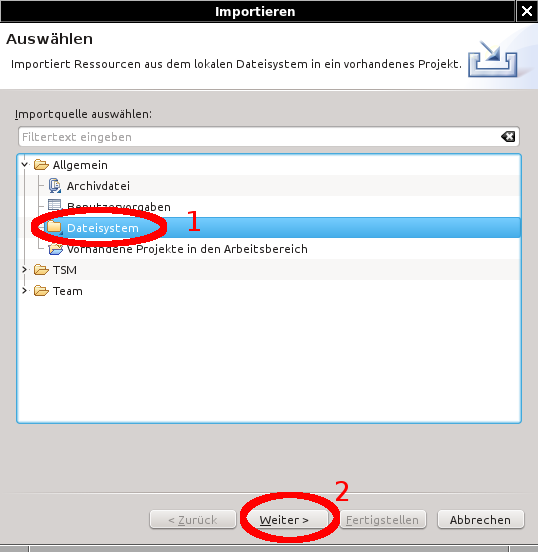
\includegraphics{./assistent-imp1.png}
 % assistent-imp1.png: 538x552 pixel, 98dpi, 13.95x14.31 cm, bb=0 0 395 406
 \caption{\texttt{Dateisystem} und dann \texttt{Weiter}.}
 \label{abb:Assistent-imp1}
\end{figure}
\vspace{\baselineskip}
Anschließend wählen Sie den gwünschten Testfall mit einem Haken aus (1) und wählen das Projekt aus (2). Beenden Sie den Import mit einem Klick auf \texttt{Fertigstellen}.
\begin{figure}[H]
 \centering
 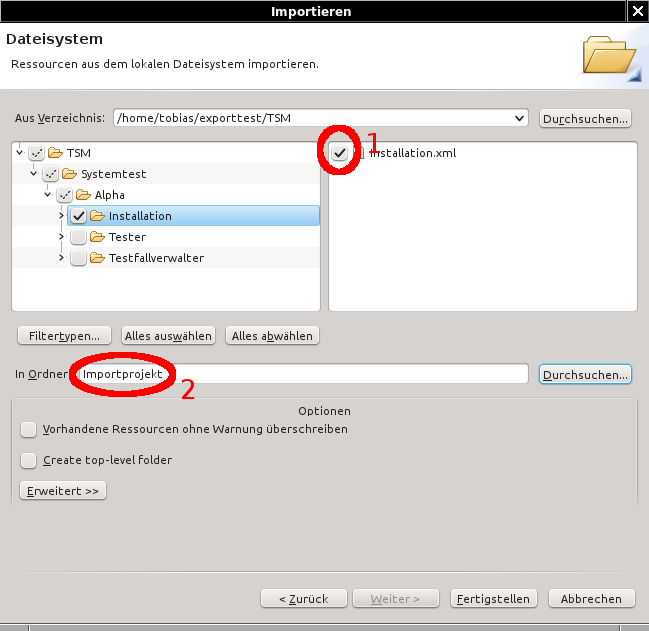
\includegraphics{./assistent-imp2.png}
 % assistent-imp2.png: 649x631 pixel, 98dpi, 16.82x16.36 cm, bb=0 0 477 464
 \caption{Haken setzen und dann das Projekt auswählen.}
 \label{abb:Assistent-imp2}
\end{figure}
\vspace{\baselineskip}
Nun sehen Sie den importierten Testfall im TSM-Navigator.
\begin{figure}[H]
 \centering
 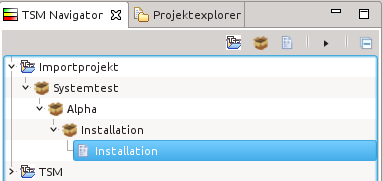
\includegraphics{./importierter-testfall.png}
 % importierter-testfall.png: 383x181 pixel, 98dpi, 9.93x4.69 cm, bb=0 0 281 133
 \caption{Der Testfall wurde erfolgreich importiert.}
 \label{abb:Importierter-testfall}
\end{figure}


\end{document}

